\documentclass{beamer}
%\documentclass[handout]{beamer}

\mode<presentation>
{
  \usetheme{CambridgeUS}
  \usefonttheme{professionalfonts}

  %\usetheme{Singapore}
  %\usecolortheme{orchid}
  %\setbeamercovered{transparent}
}

\usepackage{pgfpages}

\usepackage{alltt,verbatim,amsmath,times}
\usepackage{bm}
\usepackage[english]{babel}
\usepackage[utf8]{inputenc}
\usefonttheme[onlymath]{serif}
%\usepackage{times}
%\usepackage[T1]{fontenc}
% Or whatever. Note that the encoding and the font should match. If T1
% does not look nice, try deleting the line with the fontenc.

\usepackage{hyperref}

\newcommand{\CC}{\mathbb{C}}
\newcommand{\NN}{\mathbb{N}}
\newcommand{\RR}{\mathbb{R}}
\newcommand{\ZZ}{\mathbb{Z}}
\newcommand{\Acal}{\mathcal{A}}
\newcommand{\Bcal}{\mathcal{B}}
\newcommand{\Ccal}{\mathcal{C}}
\newcommand{\Ncal}{\mathcal{N}}
\newcommand{\Kcal}{\mathcal{K}}

\newcommand{\bF}{\mathbf{F}}
\newcommand{\bQ}{\mathbf{Q}}
\newcommand{\bU}{\mathbf{U}}
\newcommand{\bbU}{\bar{\bU}}
\newcommand{\bu}{\mathbf{u}}
\newcommand{\bv}{\mathbf{v}}

\newcommand{\Div}{\nabla\cdot}
\newcommand{\eps}{\epsilon}
\newcommand{\grad}{\nabla}
\newcommand{\lap}{\triangle}
\DeclareMathOperator{\trace}{tr}
\renewcommand{\bar}{\overline}

\newcommand{\ddx}[1]{\frac{\partial #1}{\partial x}}
\newcommand{\ddy}[1]{\frac{\partial #1}{\partial y}}
\newcommand{\pp}[2]{\frac{\partial #1}{\partial #2}}
\newcommand{\ppt}[1]{\frac{\partial #1}{\partial t}}
\newcommand{\ppT}[1]{\frac{\partial #1}{\partial T}}
\newcommand{\ppx}[1]{\frac{\partial #1}{\partial x}}
\newcommand{\ppy}[1]{\frac{\partial #1}{\partial y}}
\newcommand{\ppz}[1]{\frac{\partial #1}{\partial z}}
\newcommand{\ppxx}[1]{\frac{\partial^2 #1}{\partial x^2}}
\newcommand{\ppzz}[1]{\frac{\partial^2 #1}{\partial z^2}}

%\setbeamercolor{redtext}{fg=red!80!black}
\setbeamercolor{redtext}{fg=red!94!black}
%\setbeamercolor{greentext}{fg=green!80!black}
\setbeamercolor{greentext}{fg=green!60!black}
%\setbeamercolor{bluetext}{fg=blue!70!black}
\setbeamercolor{bluetext}{fg=blue!90!black}
\setbeamercolor{yellowtext}{fg=yellow!95!black}
\setbeamercolor{orangetext}{fg=yellow!50!red}

\newcommand{\green}{\usebeamercolor[fg]{greentext}}
\newcommand{\blue}{\usebeamercolor[fg]{bluetext}}
\newcommand{\red}{\usebeamercolor[fg]{redtext}}

\renewcommand{\L}{\emph{Left}}
\newcommand{\R}{\emph{Right}}



\title[fast flow in Greenland]{Modeled and observed fast flow in \\ the Greenland ice sheet}

\author[Bueler et al.]{Ed Bueler\inst{1} \\ \and Constantine Khroulev\inst{1} \\ \and Andy Aschwanden\inst{2} \\ \and Ian Joughin\inst{3}}

\institute[UAF and UW]{
  \tiny \inst{1}Dept of Mathematics and Statistics,
  University of Alaska Fairbanks
  \and
  \inst{2}Arctic Region Supercomputing Center,
  University of Alaska Fairbanks 
  \and  
  \inst{3}Polar Science Center, Applied Physics Lab,
  University of Washington, Seattle}

\date{}


\setbeamerfont{date}{size=\scriptsize}

\subject{ice sheet modelling, ice sheets, ice streams, parallel computing, polythermal}


%\begin{comment}
\AtBeginSection[]
{
  \begin{frame}<beamer>
    \frametitle{Outline}
    \tableofcontents[currentsection]
  \end{frame}
}
%\end{comment}


\begin{document}
\graphicspath{{figs/}}


\begin{frame}
  \titlepage
  \begin{center}
  \tiny 28 July 2009
  
  \tiny supported by NASA grants NAG5-11371 and NNX09AJ38C
  \end{center}
\end{frame}

\begin{comment}
% NO OUTLINE:
\begin{frame}
  \frametitle{Outline}
  \tableofcontents[hideallsubsections]
  % You might wish to add the option [pausesections]
\end{frame}
\end{comment}


\section{1. Observations, and modeling goals}\subsection*{}


\begin{frame}
  \frametitle{inSAR surface velocity observations}

\begin{columns}
\begin{column}{0.65\textwidth}

\begin{itemize}
\item RADARSAT SAR
\item acquired Dec 2005 to Apr 2006
%Ian says: acquired 13 Dec 2005 to 20 Apr 2006
\item inSAR and speckle-tracking to produce surface velocity\footnote{\tiny Joughin et al. [2002,2008,in preparation]} on 500 m grid
\item comparison to GPS suggests errors $<$ 10\% for $>$ 100 m/a ice; observation error much less than model error below
\item here: averaged onto 3 km grid
\item \scriptsize  method: 3 km cell is kept if at least 20\% of 500 m cells have values
\item \normalsize 71.6\% area coverage on 3 km grid
\end{itemize}
\end{column}

\begin{column}{0.35\textwidth}
  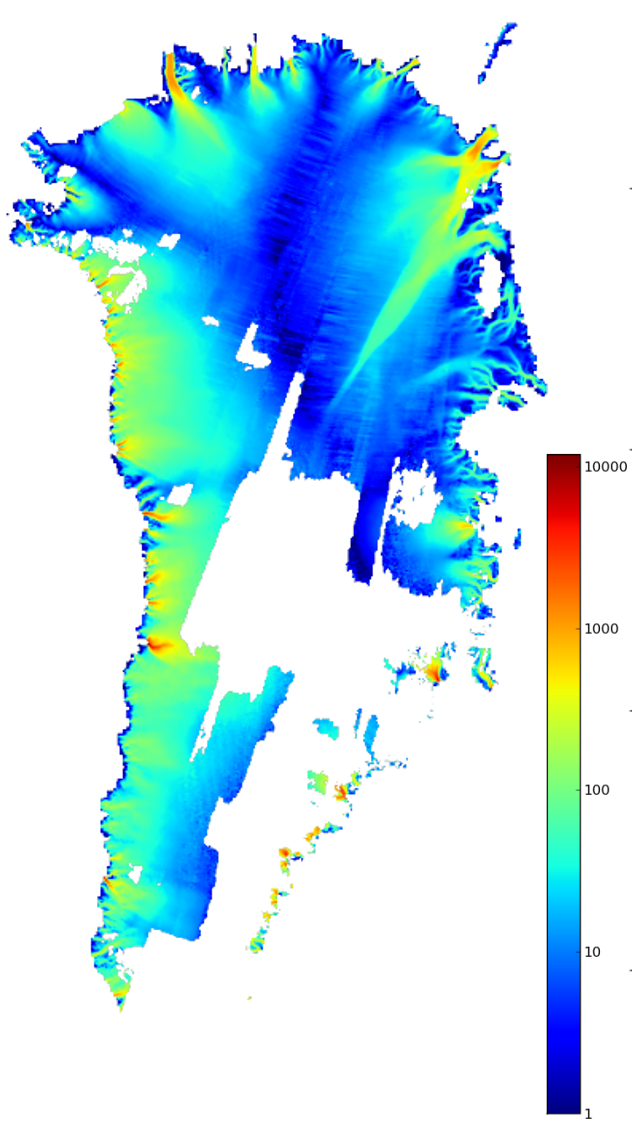
\includegraphics[width=1.0\textwidth]{joughin}
\end{column}
\end{columns}
\end{frame}


\begin{frame}
  \frametitle{``fast flow'' versus fastest flow}

\begin{itemize}
\item histogram of observed surface speed on 3 km grid $\downarrow$
\end{itemize}

\begin{columns}
\begin{column}{0.4\textwidth}
\begin{itemize}
\item exist 3 km cells with $\approx$ 12 km/a surface speed
\item \dots but few, and in tight, steep fjord topography
\item \scriptsize e.g.~only \emph{eleven} 3 km cells with average speed above 5000 m/a
\item \normalsize note log scale on $y$-axis
\item this talk: we trim off $>$ 3000 m/a cells, for comparison to whole ice sheet model
\end{itemize}
\end{column}

\begin{column}{0.6\textwidth}
  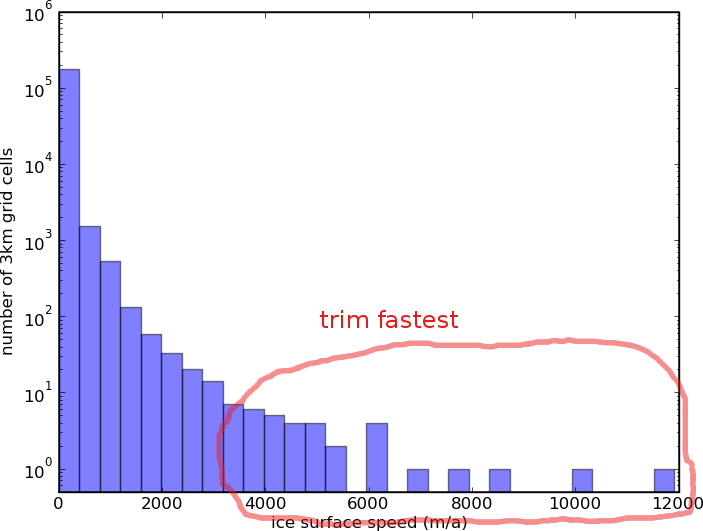
\includegraphics[width=1.0\textwidth]{joughin_histogram_to12000_trim}
\end{column}
\end{columns}
\end{frame}


\begin{frame}
  \frametitle{goal: model the fast flow}

\begin{columns}
\begin{column}{0.4\textwidth}
\begin{itemize}
\item \textbf{Definition}.  \emph{fast flow} means 100 m/a to 3000 m/a surface speed; \emph{slow} means $<$ 100 m/a
\item \textbf{Goal}: we want a model for the present dynamical state of Greenland ice sheet, with few tunable parameters, which comes close to this observed histogram $\to$
\end{itemize}
\end{column}

\begin{column}{0.6\textwidth}
  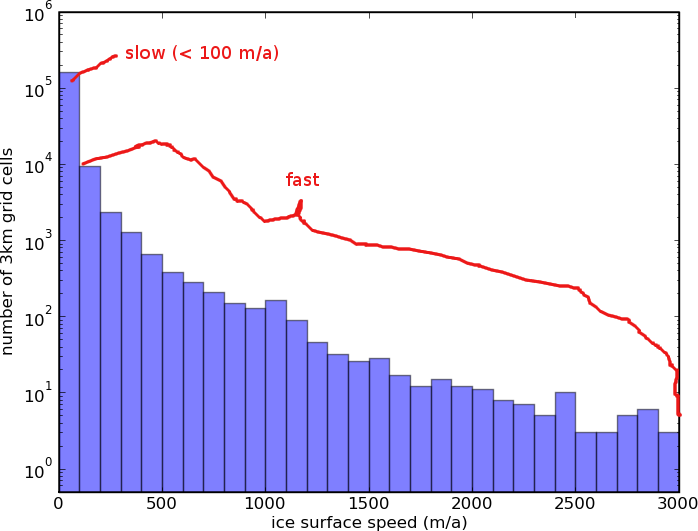
\includegraphics[width=1.0\textwidth]{joughin_histogram}
\end{column}
\end{columns}
\end{frame}

\begin{frame}
  \frametitle{goal: model the fast flow 2}

\begin{itemize}
\item why this particular goal?
  \begin{itemize} 
    \item[*] fast-flowing regions will dominate century- and millenium-scale dynamical response to climate changes
    \item[*] \dots especially sea level contribution
    \item[*] shallow models have had trouble with fast flow
    \item[*] a specific modeling goal focusses the mind
  \end{itemize} \small
\end{itemize} 
\end{frame}


\begin{frame}
  \frametitle{goal: model fast flow 3}

\begin{itemize}
\item is matching surface velocity enough?
  \begin{itemize}
  \item[*] no
  \item[*] \dots but inSAR surface velocities are the highest-dimensional existing dynamical info on the present state
  \end{itemize}
\item why not just do inverse modeling of surface velocities?
  \begin{itemize}
    \item[*] yes, we \emph{will} use inversion to get initial state for predictions
    \item[*] \dots but, for prediction and scenarios, we need a model with evolving geometry, temperature, basal resistance, etc.
  \end{itemize}

\end{itemize} 
\end{frame}


\begin{frame}
  \frametitle{the resolution challenge}

\vspace{-0.1in}

\small
\begin{itemize}
\item fast flow occurs
  \begin{itemize}
  \item[*] near, within, and over marginal mountain ranges
  \item[*] along subglacial trenches
  \end{itemize}
\item therefore shallow assumptions need to be removed
\item \emph{and} resolution needs to be high
\end{itemize} 

\begin{center}
  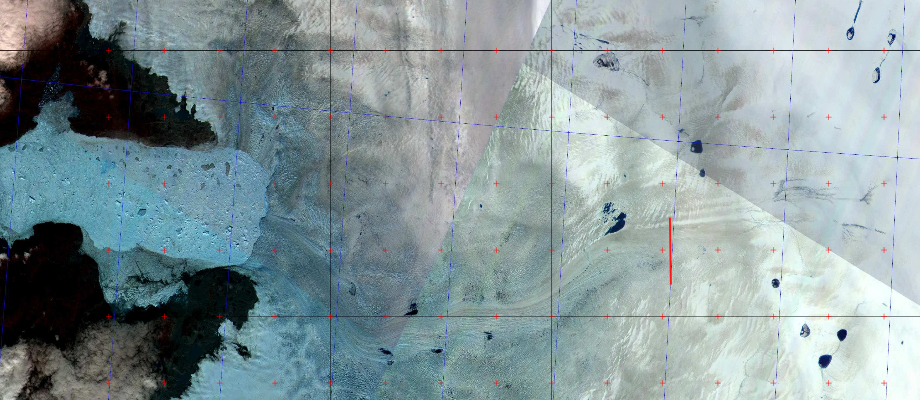
\includegraphics[width=0.7\textwidth]{jacob_5km_grid}\footnote{\tiny composite ASTER image, M.~Fahnestock and M.~Truffer}

\scriptsize  5km grid (\alert{red $+$}) and channel width (\alert{red segment}) though which much of

the Ilulissat (Jakobshavn) Glacier is fed
\end{center}
\end{frame}


\begin{frame}
  \frametitle{this talk: a small parameter study}

\begin{itemize}
\item a small parameter study\footnote{more below \dots} using a hybrid shallow model
\item results from eight whole Greenland ice sheet model runs
\item each run: 100 model years on 3 km grid
\item before start of run: spin-up in steady present climate for total of 110 k model years\footnote{\tiny On grids refining from 10 km to 5 km to 3km.  Purpose: to equilibriate ice and bedrock temperature, in balance with advection.}
\item each run starts from present bed elevation and thickness (Bamber et al 2001)
\item assumed steady, present climate:
  \begin{itemize}
  \item[*] Fausto et al. (2008) temperature parameterization
  \item[*] PARCA accumulation map (van der Veen et al. 2001)
  \item[*] positive degree day scheme for surface mass balance
  \end{itemize}
\item at end of each run: compare surface velocities to observed 
\end{itemize}
\end{frame}


\section{2. Model description}\subsection*{}

\begin{frame}
  \frametitle{shallow model ideas}

\small
\begin{itemize}
\item the Greenland ice sheet has aspect ratio $\approx 1/1000$
\item fastest-flowing parts include significant bed topography so shallow models must miss something (acknowledged!)
\item ``shallow'' models for grounded ice include
  \begin{itemize}
  \item[*] shallow ice approximation (SIA): gravity-driven lubrication flow, sticking to bed and shearing in vertical planes; \emph{no sliding in the SIA as understood here}
  \item[*] dragging shallow shelf approximation (SSA) for ice streams: gravity-driven viscous membrane sliding over variable-strength bed (``till'')
  \end{itemize}
\end{itemize}

\end{frame}


\begin{frame}
  \frametitle{shallow model ideas 2}

\vspace{-0.2in}
\begin{block}{C. Schoof (2006) insight, for diagnostic case}
$$\text{SSA + (plastic till)} = \qquad \begin{pmatrix}
\text{well-posed free boundary problem} \\ \text{for location and velocity of sliding}
\end{pmatrix} $$
\end{block}

\begin{columns}
\begin{column}{0.5\textwidth}
\begin{center}
  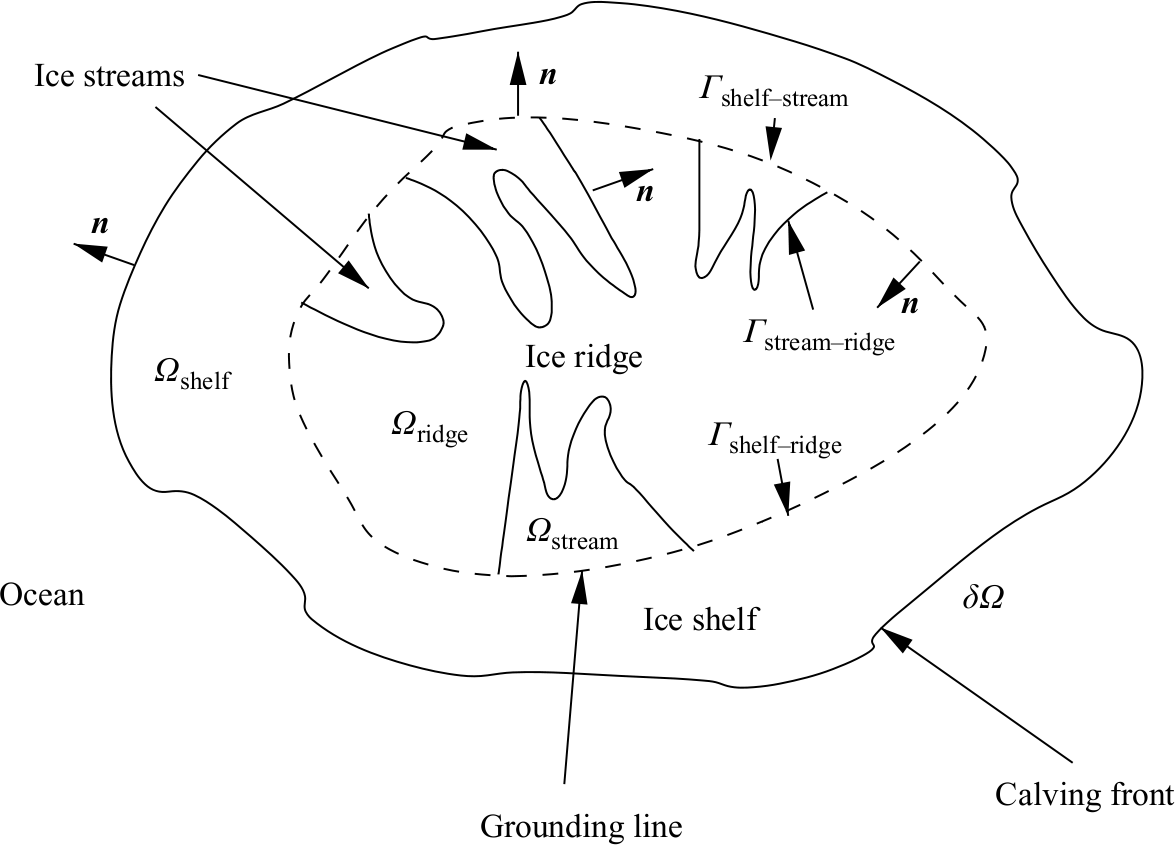
\includegraphics[width=0.75\textwidth]{schoof_planform}
\end{center}
\end{column}
\begin{column}{0.5\textwidth}
\begin{center}
  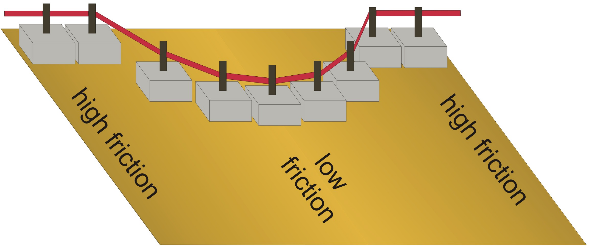
\includegraphics[width=0.75\textwidth]{schoof_sliders}
\end{center}
\end{column}
\end{columns}

\scriptsize
\begin{itemize}
\item till strength/resistance given by yield stress $\tau_c$:  \qquad $\vec\tau_b = \tau_c \mathbf{v}_b / |\mathbf{v}_b|$
\item scheme is a whole ice sheet form of D.~MacAyeal's individual ice stream models (1989)
\end{itemize}
\end{frame}



\begin{frame}
  \frametitle{Parallel Ice Sheet Model (PISM)}

\begin{itemize}
\item SIA and SSA velocity solutions, combined or separate
\item thermomechanically-coupled
\item parallel:
  \begin{itemize}
  \item[*] 3 km grid runs here done on 64, 128, or 256 processors at Arctic Region Supercomputing Center, Fairbanks
  \item[*] $501 \times 935 \times 201$ ice grid; $\approx$ 300 million temperature and velocity unknowns
  \item[*] all runs here total $\approx$ 8000 processor-hours
  \item[*] is that a lot of processor-hours?
  \end{itemize}
\item homepage\qquad \texttt{www.pism-docs.org}
\end{itemize}
\end{frame}


\begin{frame}
  \frametitle{PISM: Schoof ideas adapted to prognostic modeling}

\begin{columns}
\begin{column}{0.6\textwidth}

\begin{itemize}
\item SSA-as-a-sliding law \scriptsize (Bueler et al. 2009) \normalsize
  \begin{itemize}
  \item[*] $\mathbf{U} = f(|\mathbf{v}|) \mathbf{u} + \left(1-f(|\mathbf{v}|)\right) \mathbf{v}$, where
  \item[*] $\mathbf{v}$ is SSA solution
  \item[*] $\mathbf{u}$ is SIA solution
  \item[*] $\mathbf{U}$ is model velocity used in mass continuity and energy conservation equations
  \end{itemize}

\end{itemize}
\end{column}

\begin{column}{0.4\textwidth}
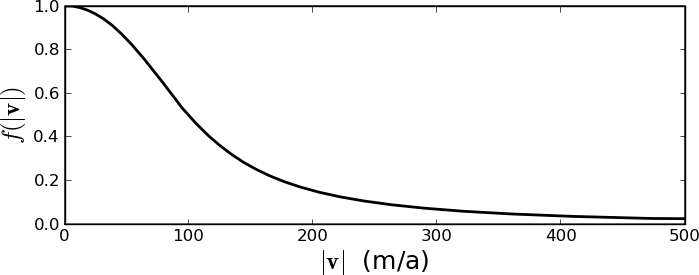
\includegraphics[width=1.0\textwidth]{fofv}
\end{column}
\end{columns}

\begin{itemize}
\item pseudo-plasticity:
	$$\vec \tau_b = \tau_c \frac{\mathbf{v}_b}{|\mathbf{v}_b|^{1-q} (100 \text{ m/a})^q}$$
\item surround ice sheet by thin notional ice shelf to maintain ellipticity of SSA
\end{itemize}
\end{frame}


\begin{frame}
  \frametitle{PISM: (\textsl{newly}!) polythermal by enthalpy method}

\begin{itemize}
\item Aschwanden and Blatter (2008 JGR; in preparation 2009)
\item $E$=enthalpy=(sensible thermal $+$ latent thermal $+$ potential of pressure)
\item temperature $T$ and liquid water fraction $\omega$ are functions of enthalpy and pressure, for cold and temperate ice: 
  $$T=T(E,p), \qquad \omega=\omega(E,p)$$
\item \emph{think}: $E=E(t,x,y,z)$ is the primal thermal variable in conservation of energy equation
\item solve conservation of energy equation for $E$
\end{itemize}

\end{frame}


\begin{frame}
  \frametitle{PISM: basal thermo-mechanical model}

\begin{itemize}
\item yield stress determined by Mohr-Coulomb:
	$$\tau_c = c_0 + (\tan \phi)\left(\rho g H - p_w\right)$$
\item $c_0=0$
\item basal melt rate from 1 \% $\omega$ rule (Greve 1997)
\item pore water pressure $p_w$ is local, time-integrated function of basal melt rate
\item till friction angle $\phi$ determined by bed elevation below sea level
  \begin{itemize}
  \item[*] motivated by presumed marine history of sediment below sea level (Huybrechts and de Wolde 1999)
  \item[*] $\phi=5^\circ$ at -700 m and below
  \item[*] $\phi=20^\circ$ at +300 m and above
  \item[*] linear between
  \end{itemize}
\item \alert{model description done!}
\end{itemize}
\end{frame}



\section{3. Results}\subsection*{}

\begin{frame}
  \frametitle{parameter study: control run plus six variations}

\begin{center}
  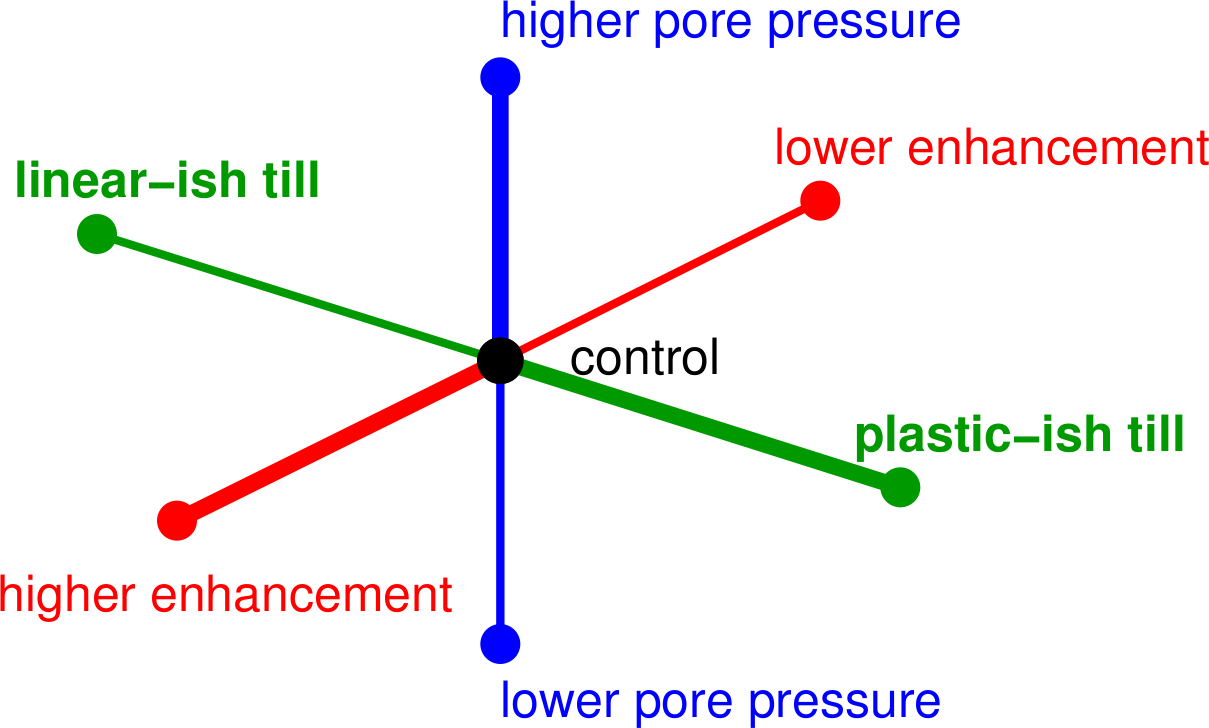
\includegraphics[width=0.5\textwidth]{param_axes}
\end{center}

\small
\begin{itemize}
\item {\red enhancement factor $e$: 1,} 3 {\red , 5} 
\item {\green exponent $q$ in basal power law; $0$=plastic, $1$=linear: 0.50,} 0.25 {\green , 0.10} 
\item {\blue limit $p_{\text{max}}$ on pore water pressure; \% of overburden: 95,} 98 {\blue , 99} 
\scriptsize
\item  first directly affects only SIA velocities, last two directly affect only SSA velocities
\end{itemize}
\end{frame}


\begin{frame}
  \frametitle{Control run results}

\begin{columns}
\begin{column}{0.6\textwidth}
\scriptsize
\begin{itemize}
\item enhancement factor=3, limit on pore water pressure=98\%, exponent in basal power law=0.25
\end{itemize}
\begin{center}
  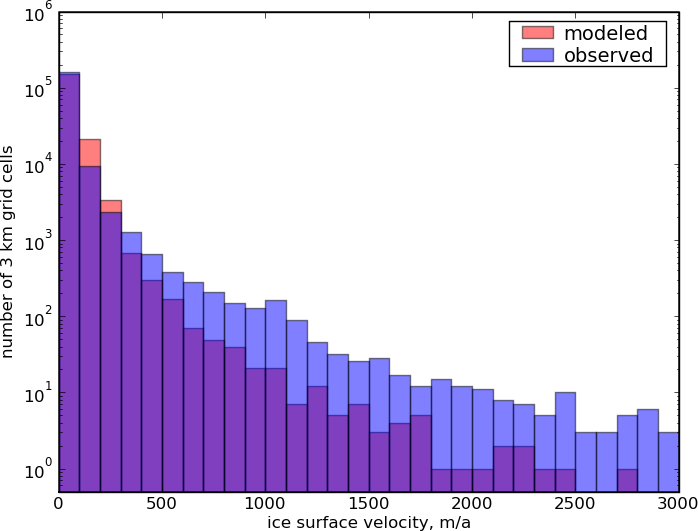
\includegraphics[width=1.0\textwidth]{g3km_3_25_98_hist}
\end{center}
\end{column}
\begin{column}{0.4\textwidth}
\begin{center}
  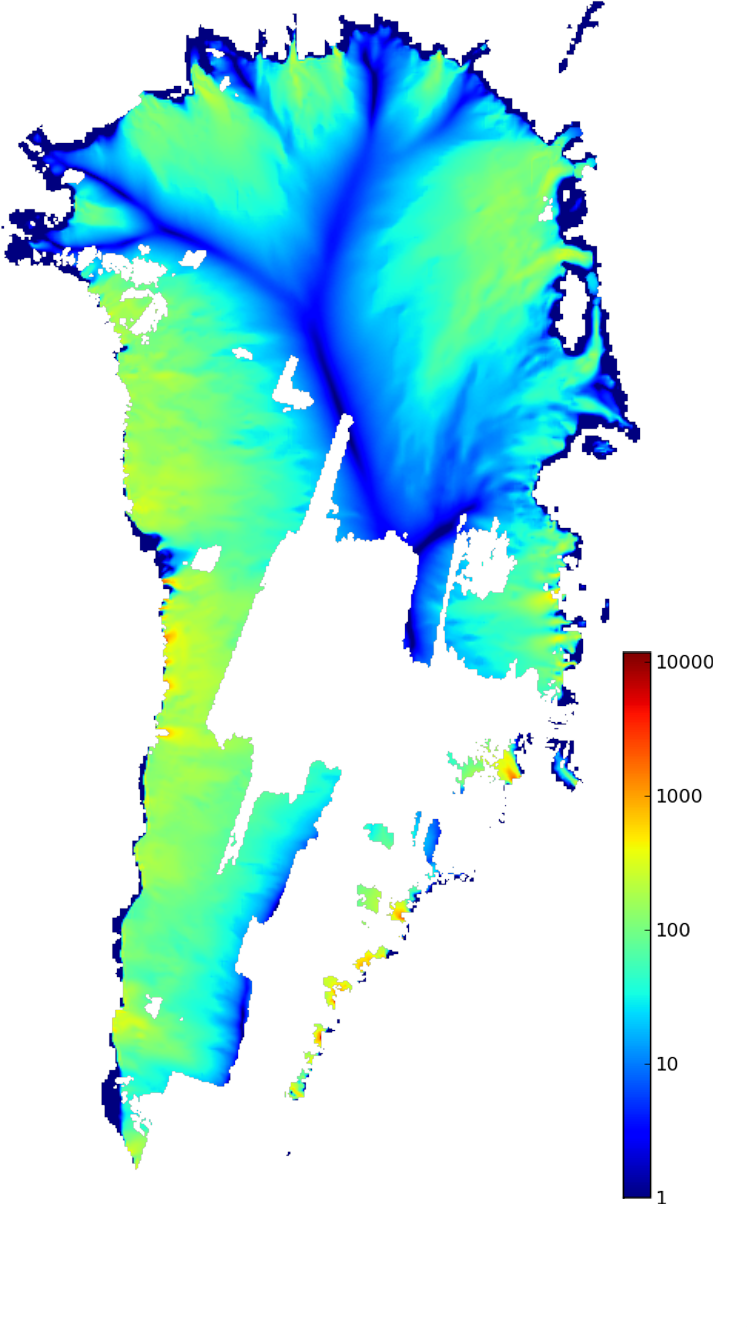
\includegraphics[width=0.75\textwidth]{g3km_3_25_98}
\end{center}
\end{column}
\end{columns}
\end{frame}


\begin{frame}
  \frametitle{Control run results 2: how much is from sliding?}

\begin{columns}
\begin{column}{0.6\textwidth}
\begin{itemize}
\item sliding speed, on same velocity scale $\to$
\end{itemize}
\end{column}
\begin{column}{0.4\textwidth}
\begin{center}
  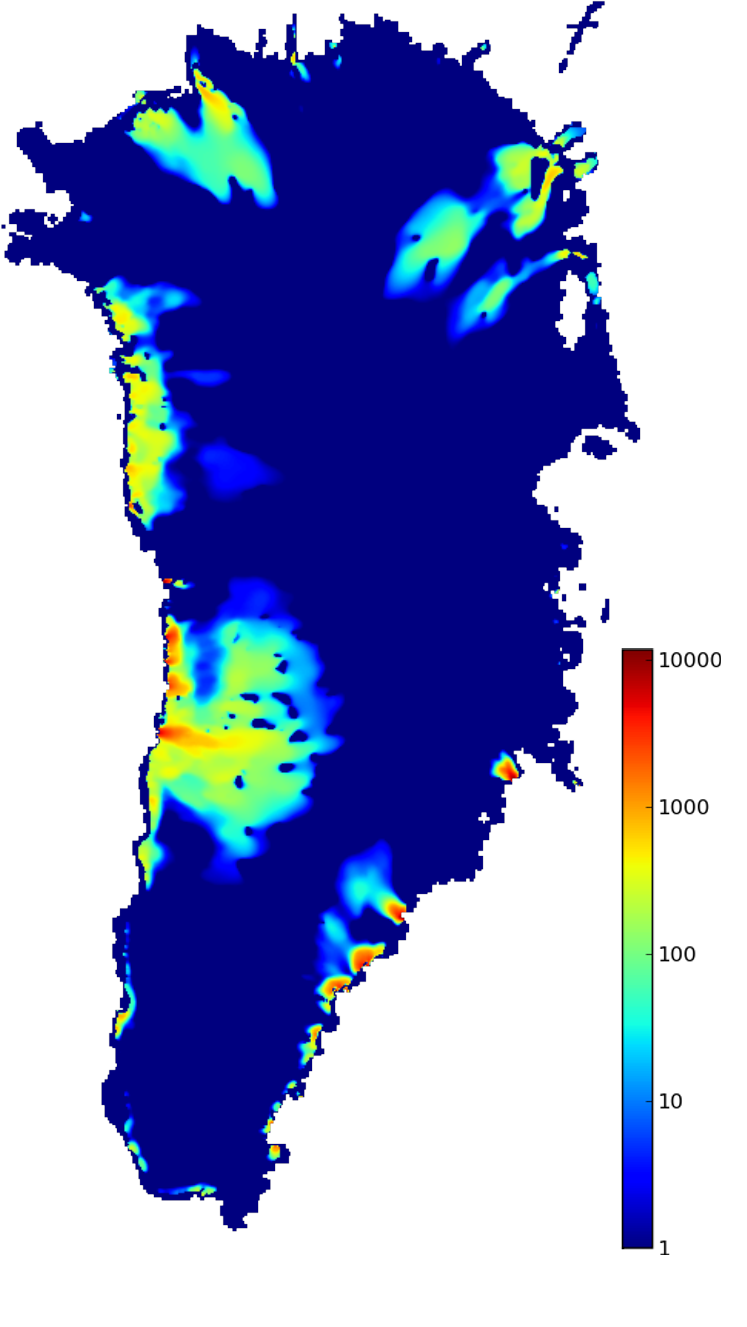
\includegraphics[width=0.75\textwidth]{g3km_3_25_98_cbase}
\end{center}
\end{column}
\end{columns}
\end{frame}


\begin{frame}
  \frametitle{Control run results 3: what if there is no sliding at all?}

\begin{columns}
\begin{column}{0.6\textwidth}
\scriptsize
\begin{itemize}
\item enhancement factor=3 and no SSA computation (no sliding; SIA only; ``sub-control'' run?)
\item \alert{SIA-only models with no sliding give reasonable distribution of fast flow}, if done on 3 km grid
\item distinction from with-SSA-sliding runs seen in time-dependence \dots another talk \dots
\end{itemize}
\vspace{-0.18in}

\begin{center}
  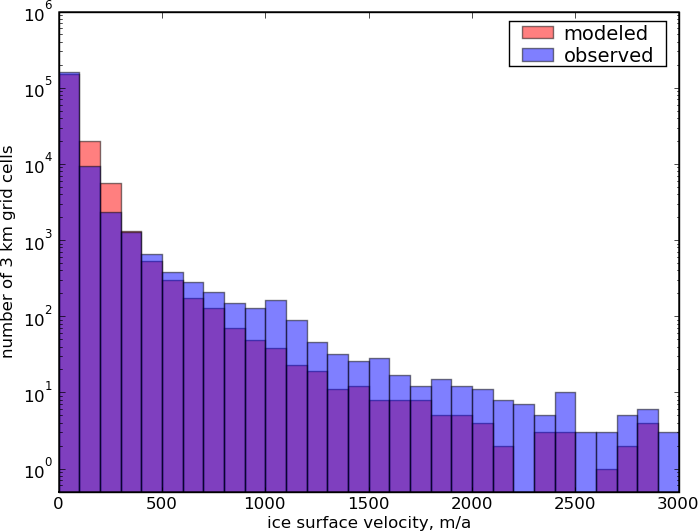
\includegraphics[width=0.9\textwidth]{g3km_3_SIA_hist}
\end{center}
\end{column}
\begin{column}{0.4\textwidth}
\begin{center}
  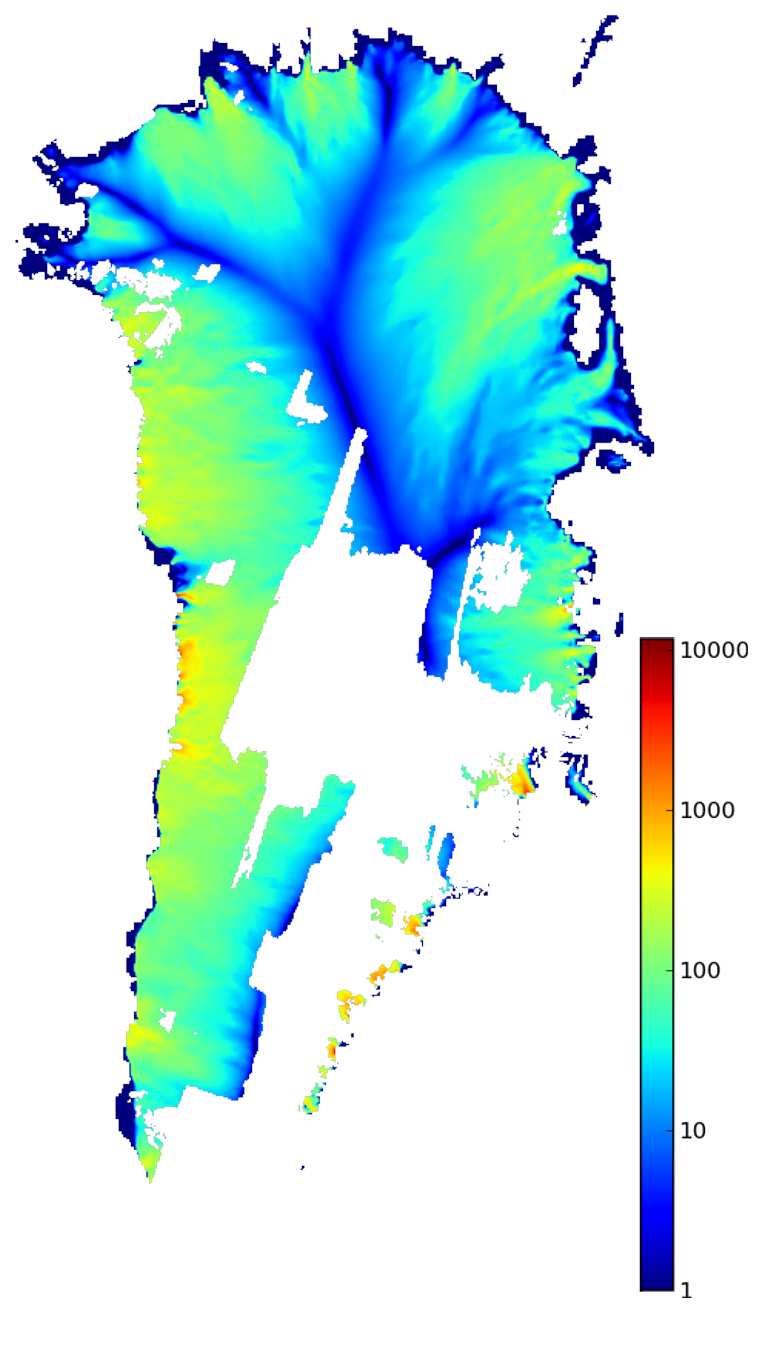
\includegraphics[width=0.75\textwidth]{g3km_3_SIA}
\end{center}
\end{column}
\end{columns}
\end{frame}


\begin{frame}
  \frametitle{Enhancement factor axis}

\vspace{-0.1in}
\begin{center}
  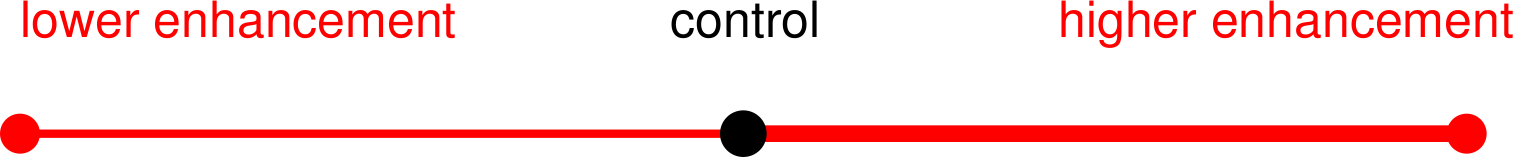
\includegraphics[width=0.6\textwidth]{enhancement_axis}
\end{center}

\vspace{-0.1in}
\begin{columns}
\begin{column}{0.33\textwidth}
\begin{center}
  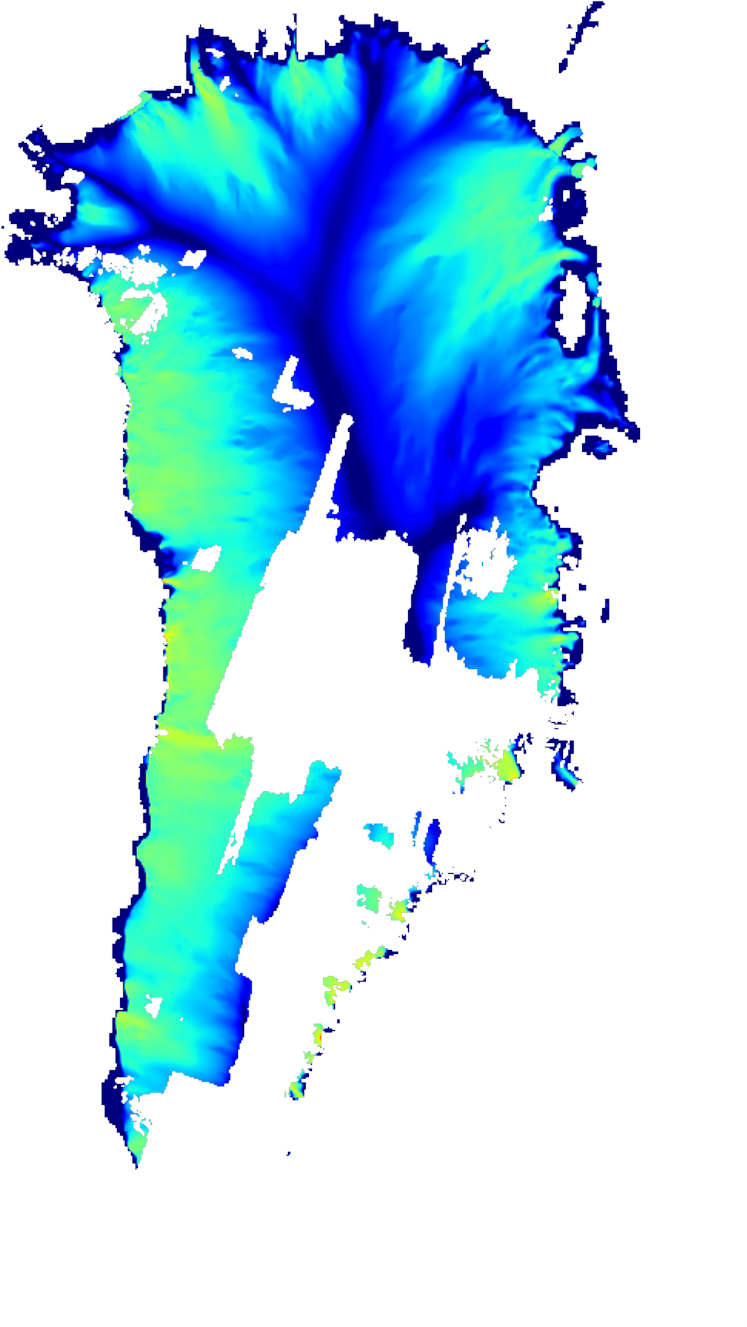
\includegraphics[width=0.85\textwidth]{g3km_1_25_98}
\end{center}
\end{column}
\begin{column}{0.33\textwidth}
\begin{center}
  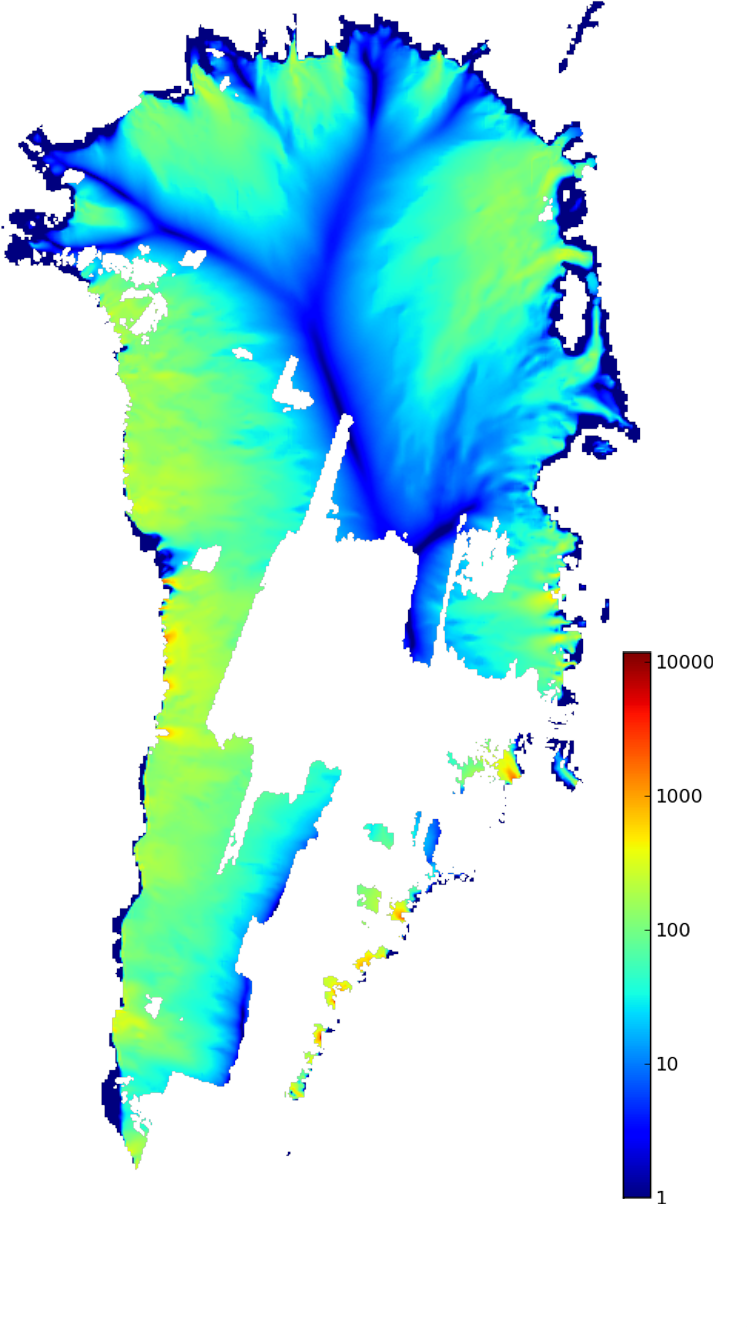
\includegraphics[width=0.85\textwidth]{g3km_3_25_98}
\end{center}
\end{column}
\begin{column}{0.33\textwidth}
\begin{center}
  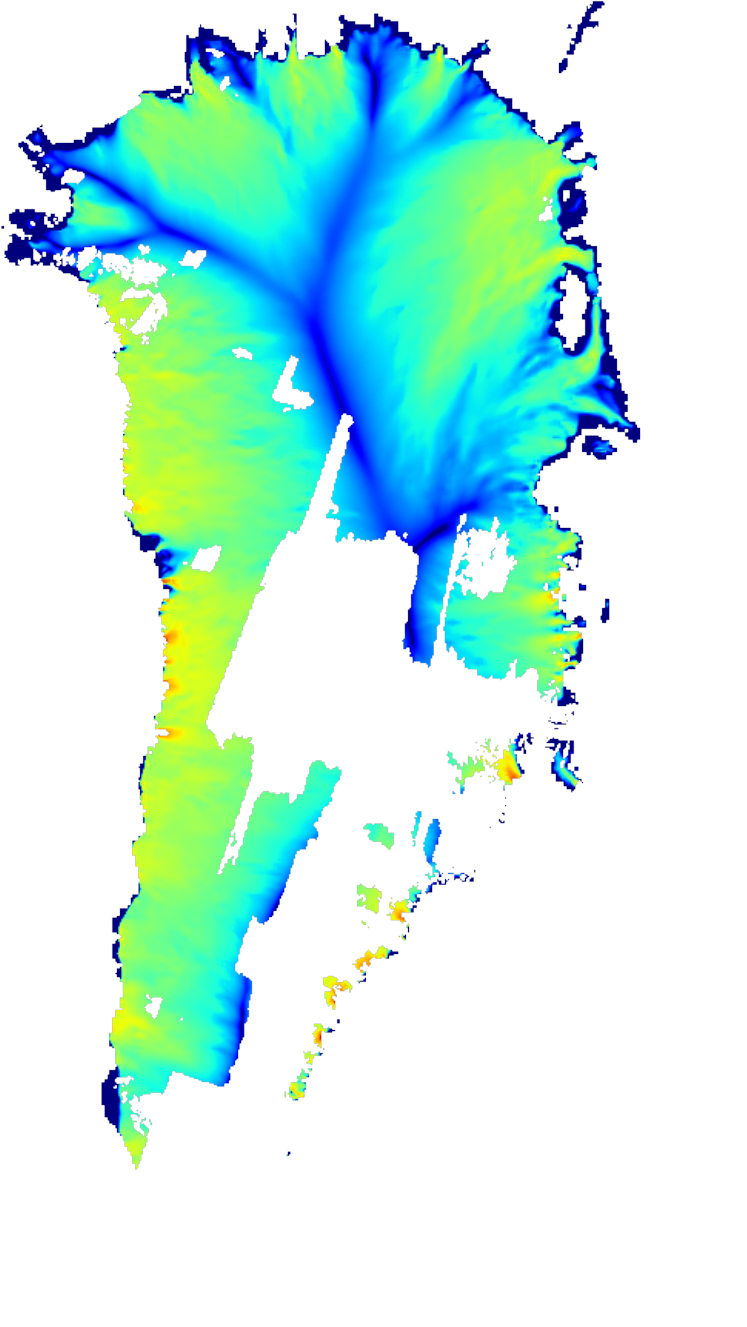
\includegraphics[width=0.85\textwidth]{g3km_5_25_98}
\end{center}
\end{column}
\end{columns}
\end{frame}

\begin{frame}
  \frametitle{Enhancement factor axis 2}

\vspace{-0.1in}
\begin{center}
  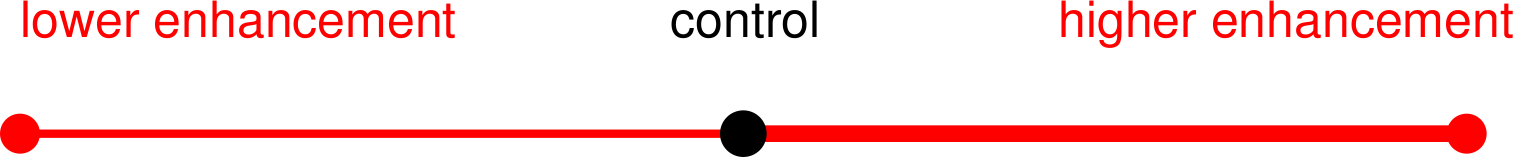
\includegraphics[width=0.6\textwidth]{enhancement_axis}
\end{center}

\vspace{-0.1in}
\begin{columns}
\begin{column}{0.33\textwidth}
\begin{center}
  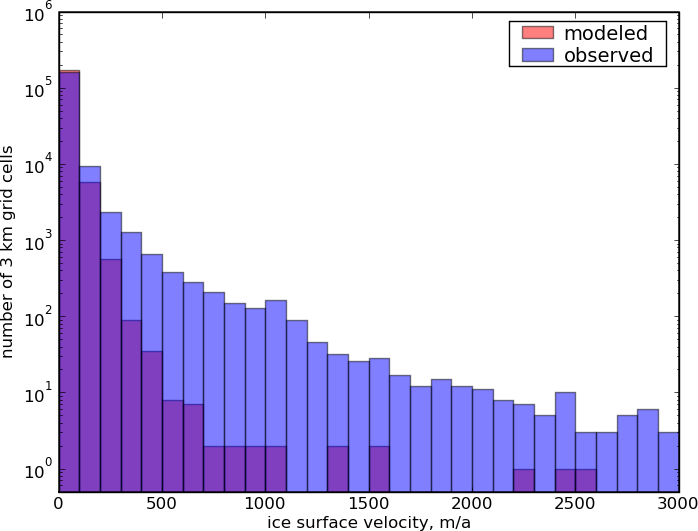
\includegraphics[width=1.0\textwidth]{g3km_1_25_98_hist}
\end{center}
\end{column}
\begin{column}{0.33\textwidth}
\begin{center}
  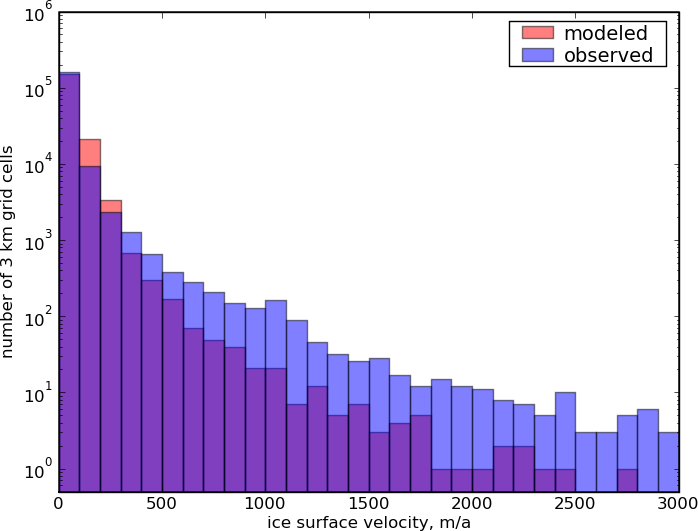
\includegraphics[width=1.0\textwidth]{g3km_3_25_98_hist}
\end{center}
\end{column}
\begin{column}{0.33\textwidth}
\begin{center}
  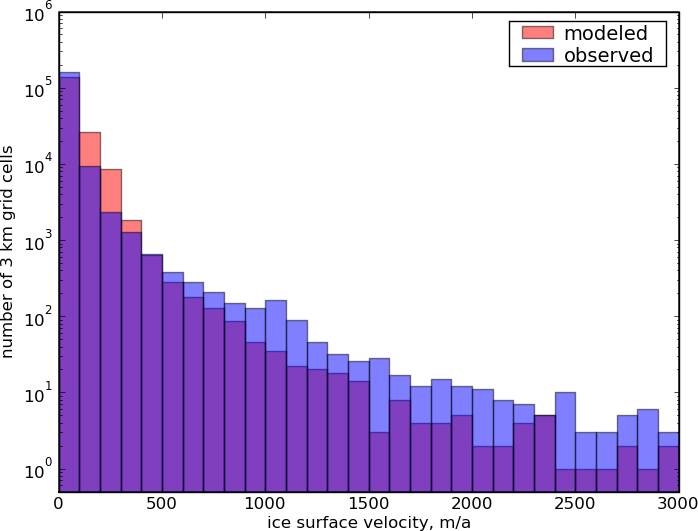
\includegraphics[width=1.0\textwidth]{g3km_5_25_98_hist}
\end{center}
\end{column}
\end{columns}
\end{frame}

\begin{frame}
  \frametitle{Allowed pore water pressure axis}

\vspace{-0.1in}
\begin{center}
  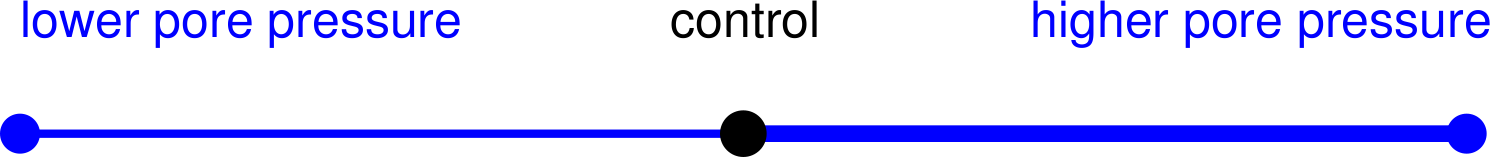
\includegraphics[width=0.6\textwidth]{pore_pressure_axis}
\end{center}

\vspace{-0.1in}
\begin{columns}
\begin{column}{0.33\textwidth}
\begin{center}
  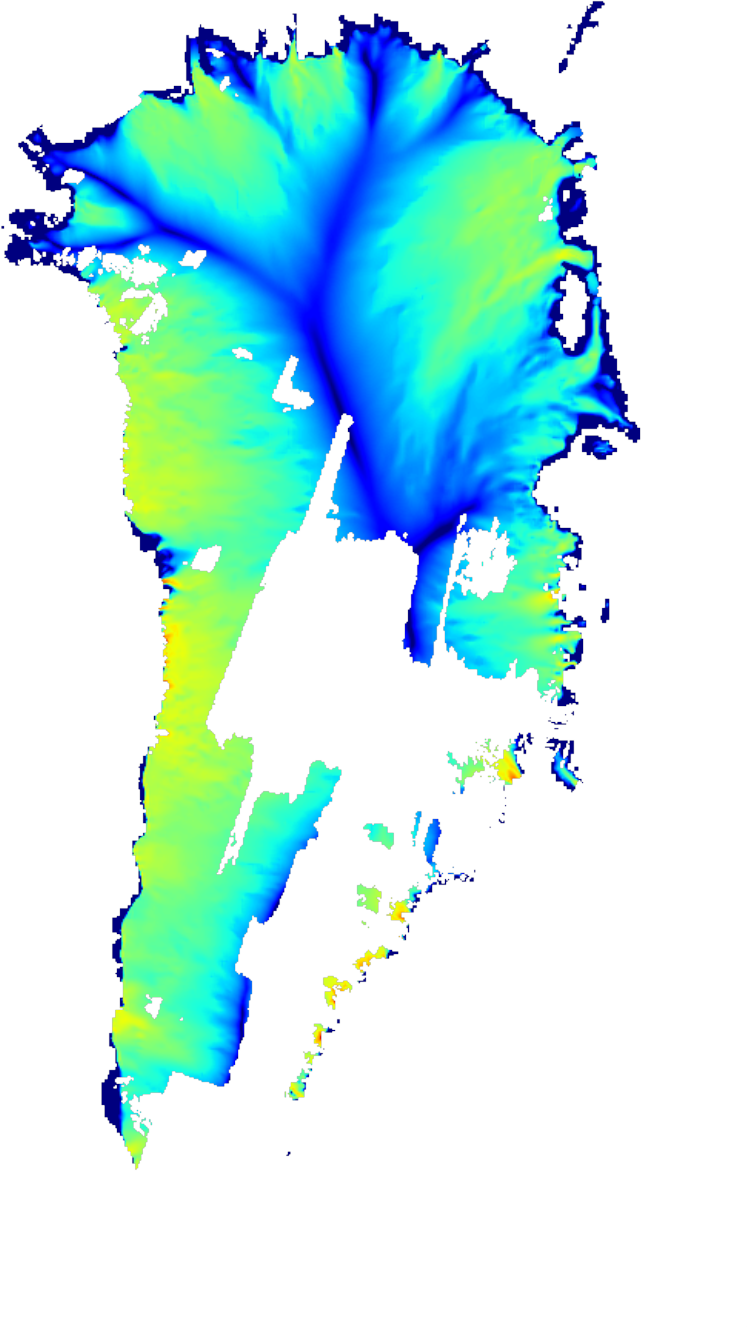
\includegraphics[width=0.85\textwidth]{g3km_3_25_95}
\end{center}
\end{column}
\begin{column}{0.33\textwidth}
\begin{center}
  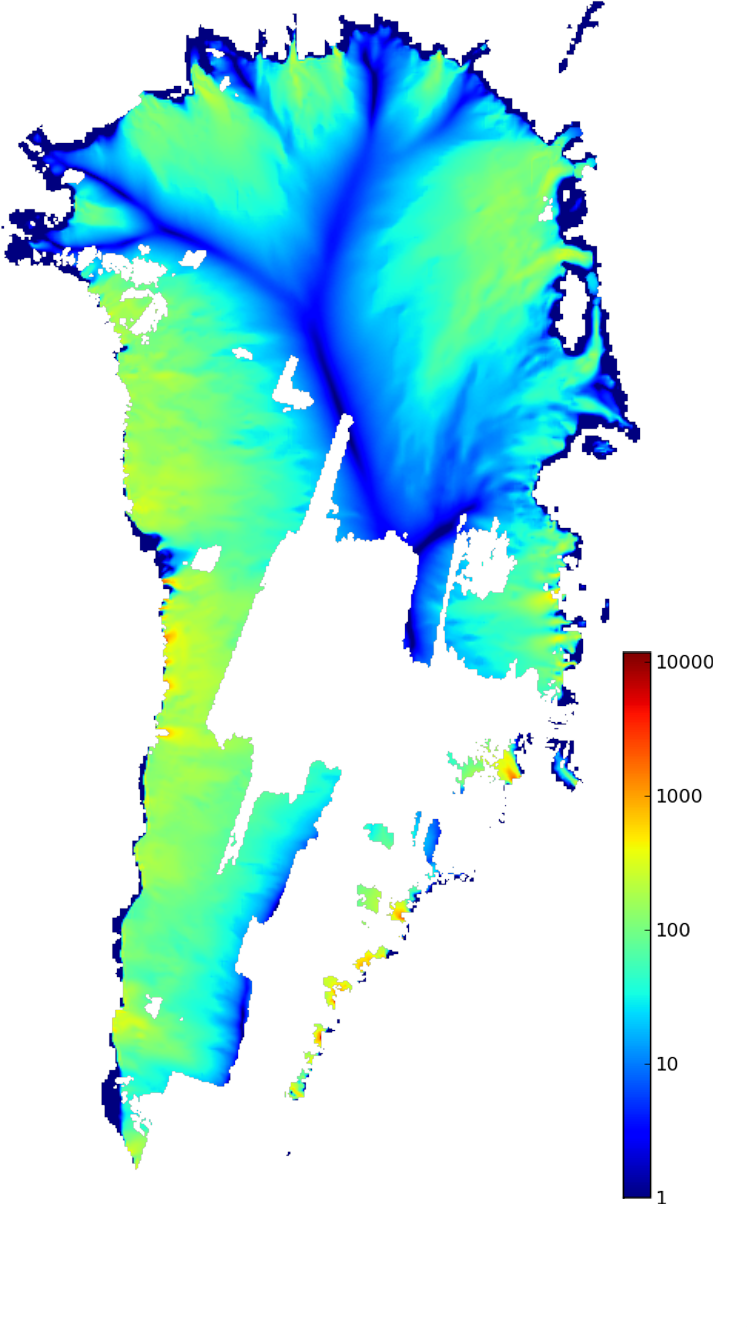
\includegraphics[width=0.85\textwidth]{g3km_3_25_98}
\end{center}
\end{column}
\begin{column}{0.33\textwidth}
\begin{center}
  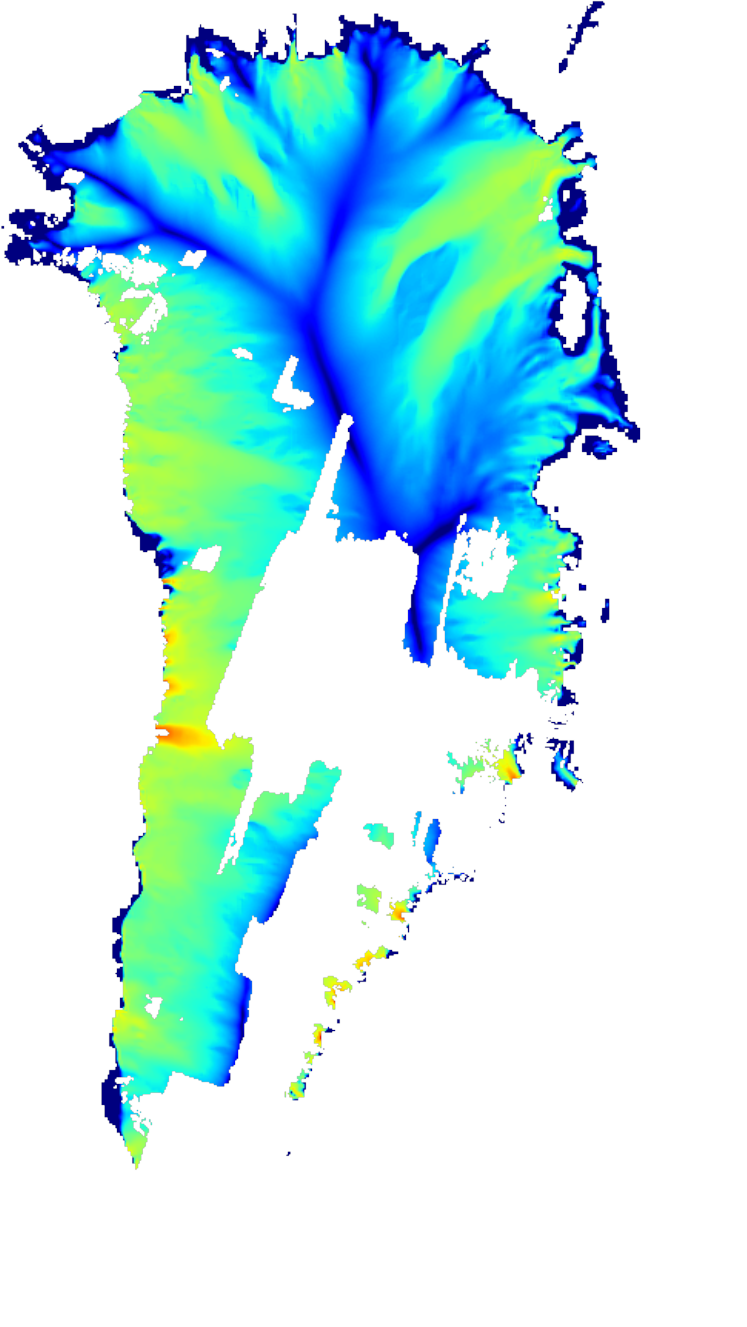
\includegraphics[width=0.85\textwidth]{g3km_3_25_99}
\end{center}
\end{column}
\end{columns}
\end{frame}


\begin{frame}
  \frametitle{Allowed pore water pressure axis 2}

\vspace{-0.1in}
\begin{center}
  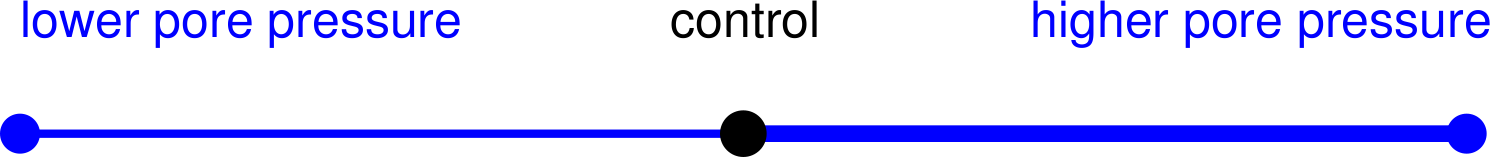
\includegraphics[width=0.6\textwidth]{pore_pressure_axis}
\end{center}

\vspace{-0.1in}
\begin{columns}
\begin{column}{0.33\textwidth}
\begin{center}
  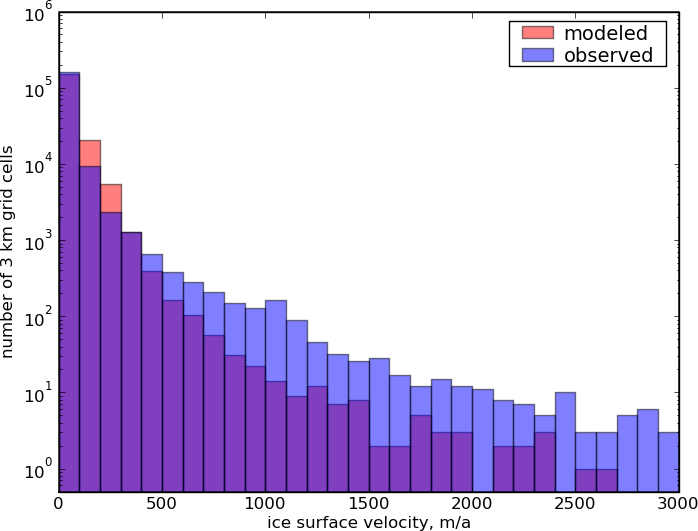
\includegraphics[width=1.0\textwidth]{g3km_3_25_95_hist}
\end{center}
\end{column}
\begin{column}{0.33\textwidth}
\begin{center}
  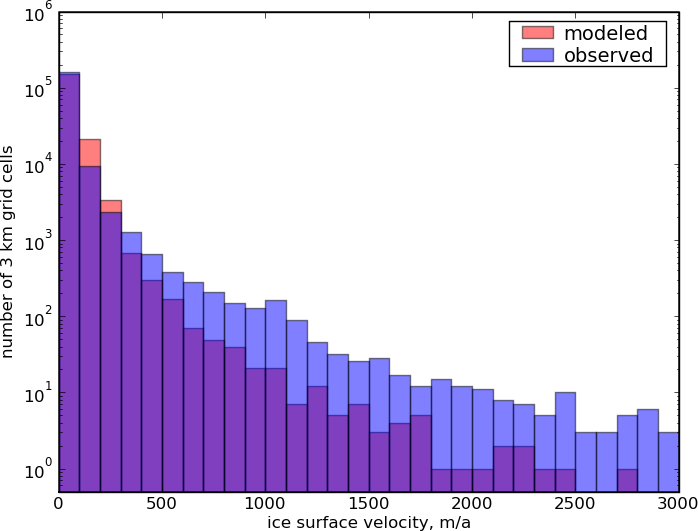
\includegraphics[width=1.0\textwidth]{g3km_3_25_98_hist}
\end{center}
\end{column}
\begin{column}{0.33\textwidth}
\begin{center}
  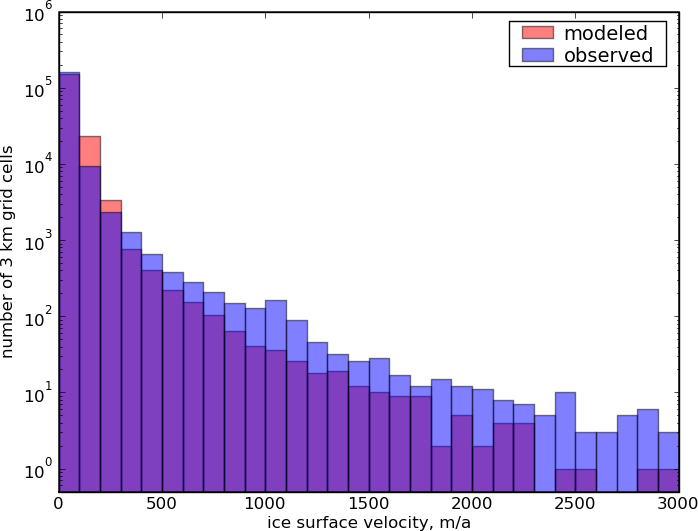
\includegraphics[width=1.0\textwidth]{g3km_3_25_99_hist}
\end{center}
\end{column}
\end{columns}
\end{frame}


\begin{frame}
  \frametitle{Plasticity (power law power) axis}

\vspace{-0.1in}
\begin{center}
  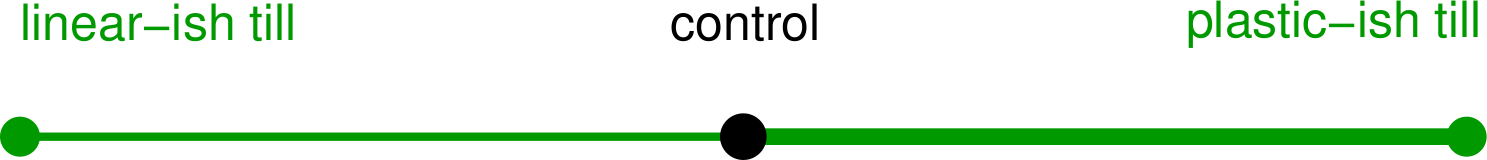
\includegraphics[width=0.6\textwidth]{plastic_axis}
\end{center}

\vspace{-0.1in}
\begin{columns}
\begin{column}{0.33\textwidth}
\begin{center}
  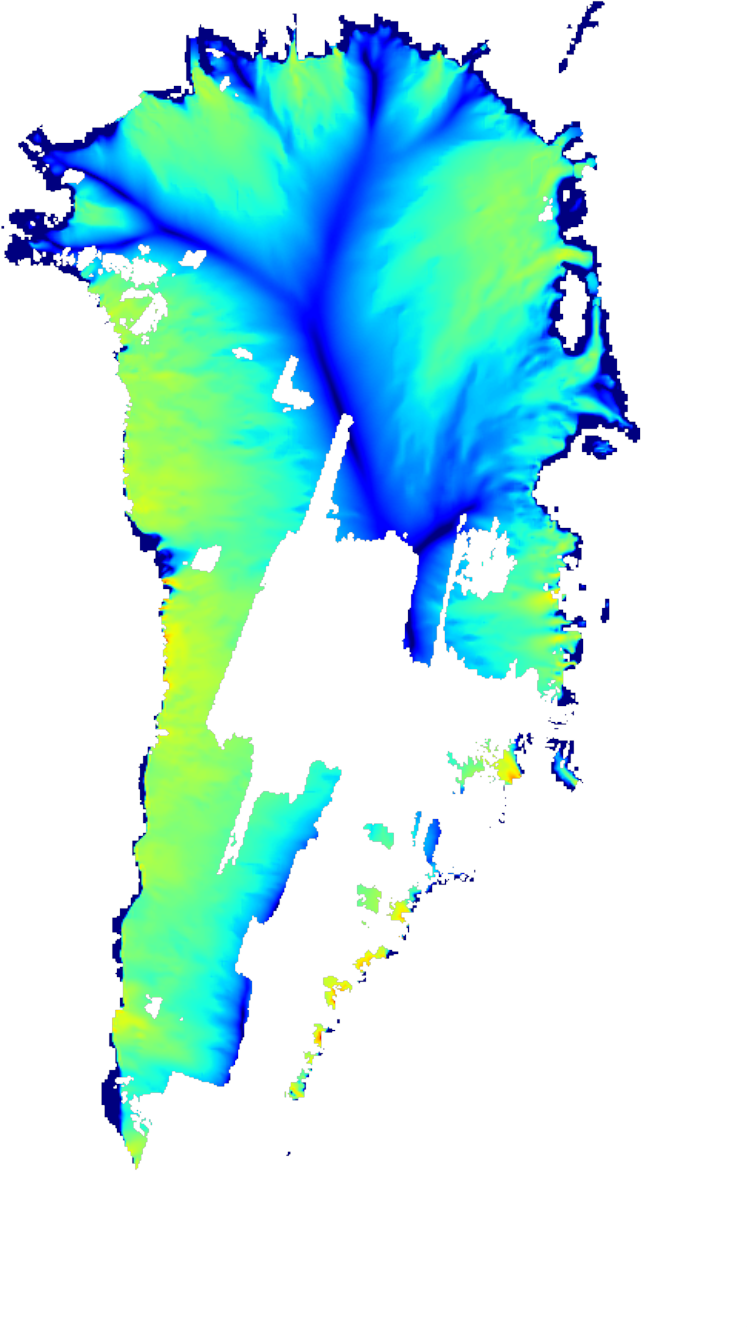
\includegraphics[width=0.85\textwidth]{g3km_3_50_98}
\end{center}
\end{column}
\begin{column}{0.33\textwidth}
\begin{center}
  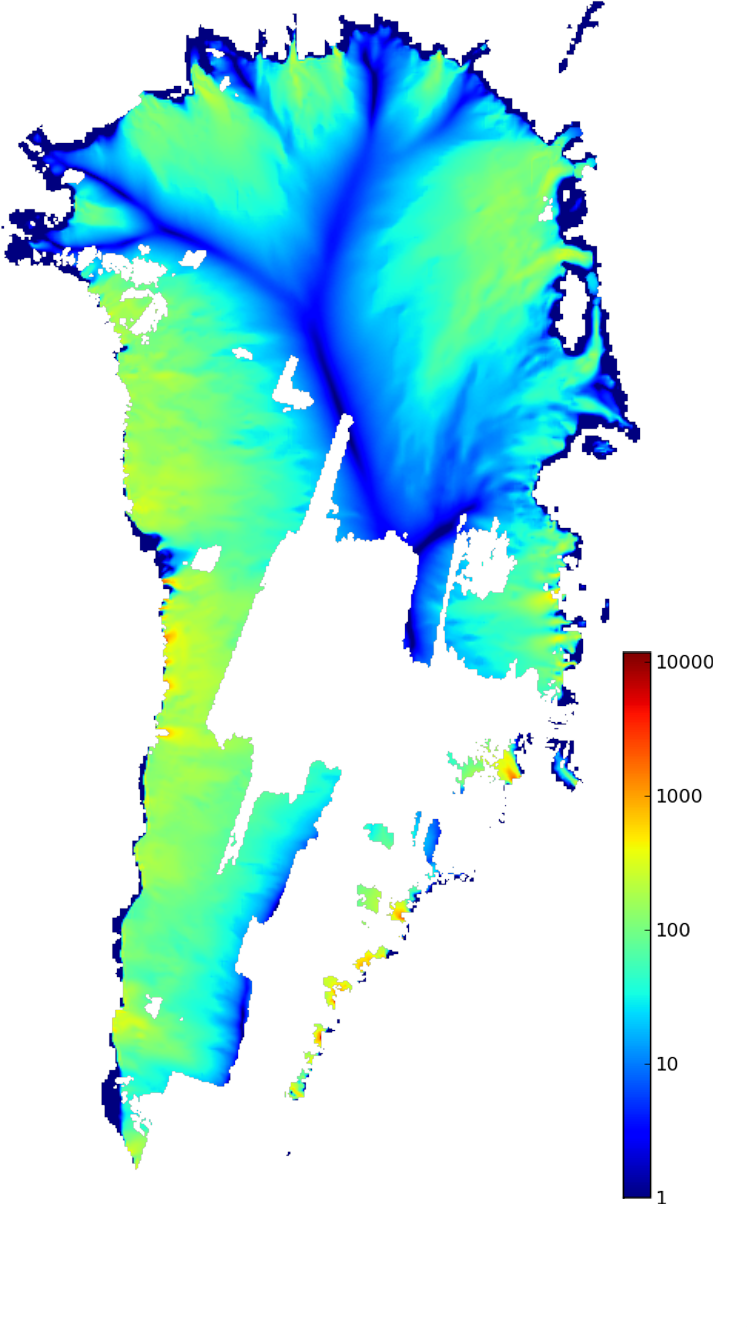
\includegraphics[width=0.85\textwidth]{g3km_3_25_98}
\end{center}
\end{column}
\begin{column}{0.33\textwidth}
\begin{center}
  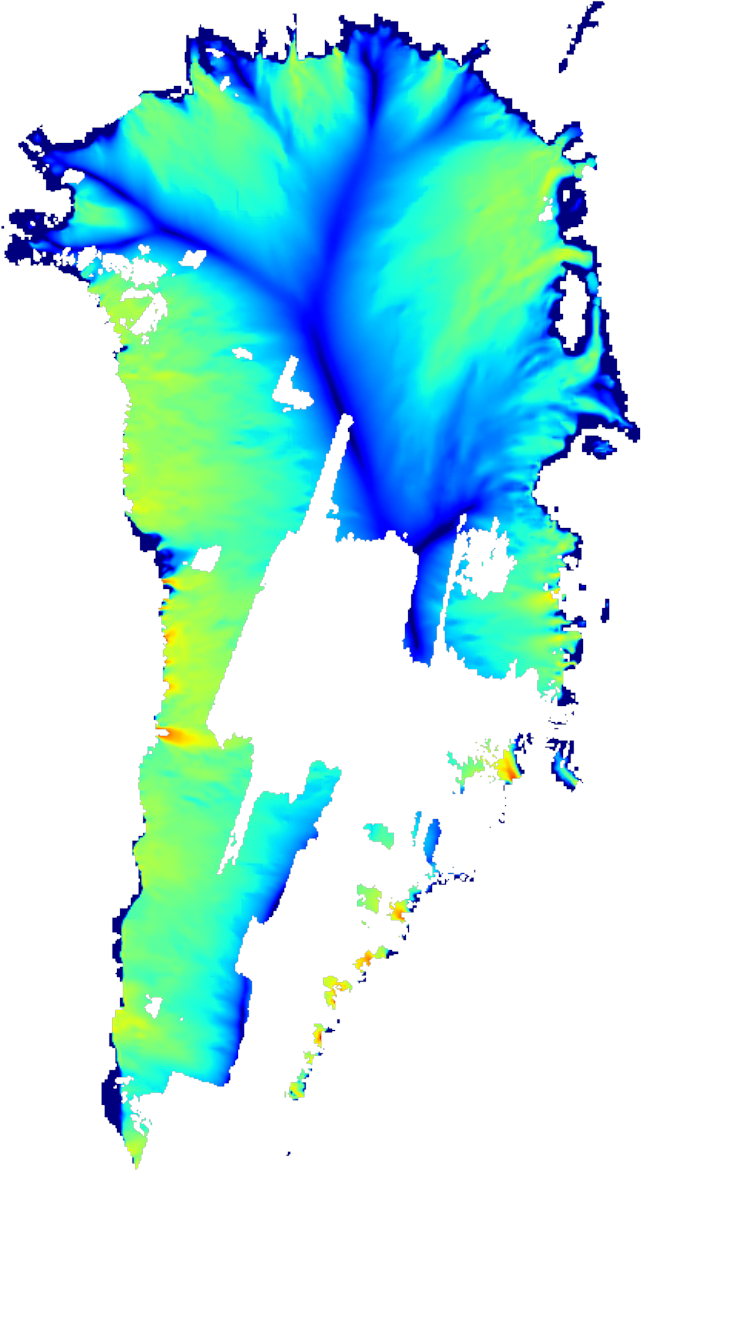
\includegraphics[width=0.85\textwidth]{g3km_3_10_98}
\end{center}
\end{column}
\end{columns}
\end{frame}


\begin{frame}
  \frametitle{Plasticity (power law power) axis 2}

\vspace{-0.1in}
\begin{center}
  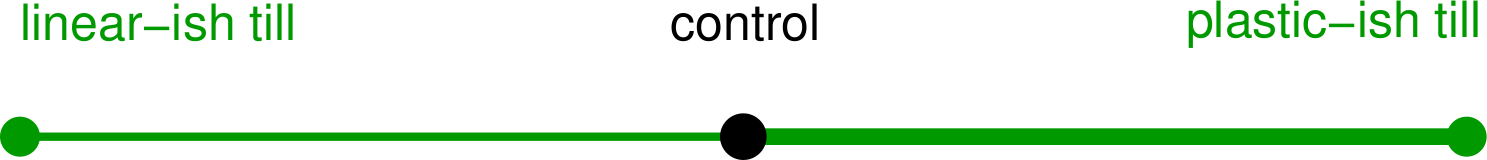
\includegraphics[width=0.6\textwidth]{plastic_axis}
\end{center}

\vspace{-0.1in}
\begin{columns}
\begin{column}{0.33\textwidth}
\begin{center}
  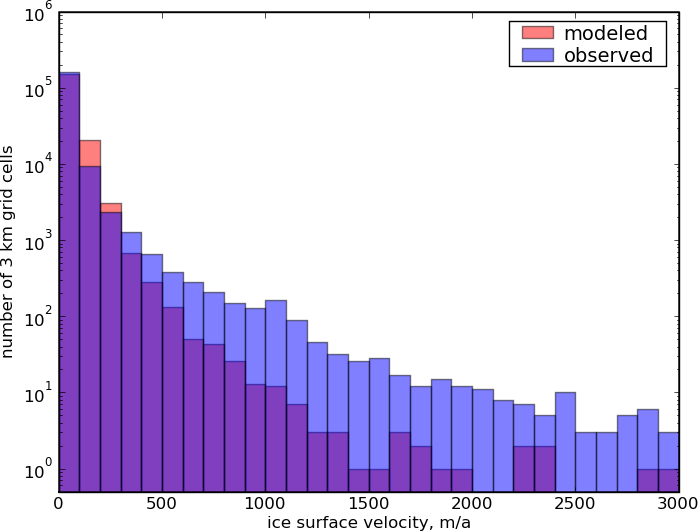
\includegraphics[width=1.0\textwidth]{g3km_3_50_98_hist}
\end{center}
\end{column}
\begin{column}{0.33\textwidth}
\begin{center}
  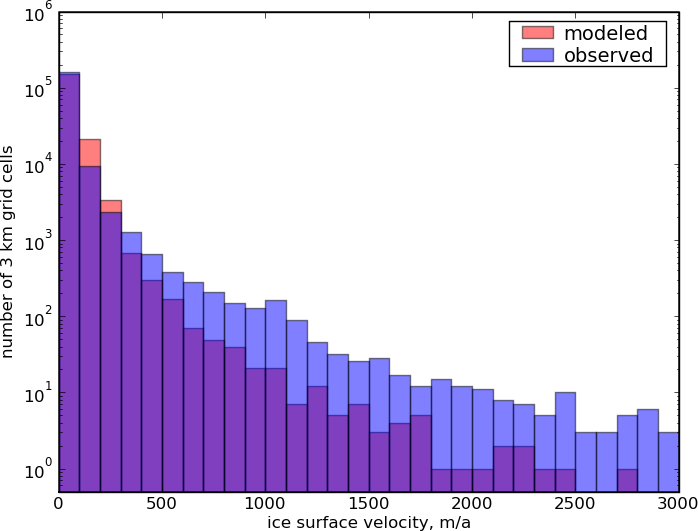
\includegraphics[width=1.0\textwidth]{g3km_3_25_98_hist}
\end{center}
\end{column}
\begin{column}{0.33\textwidth}
\begin{center}
  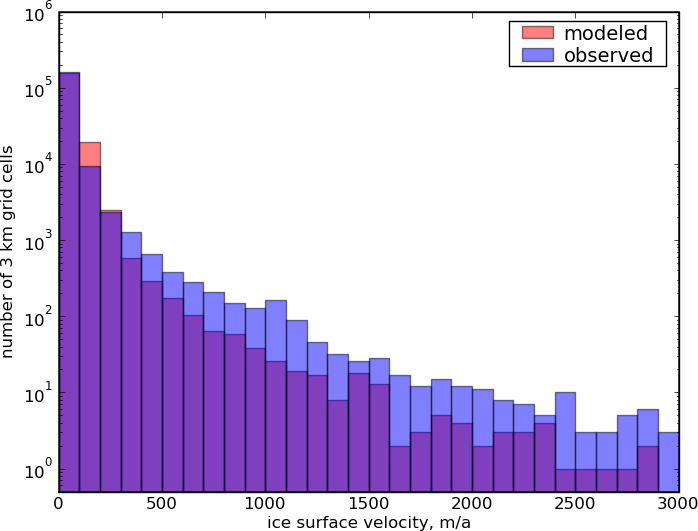
\includegraphics[width=1.0\textwidth]{g3km_3_10_98_hist}
\end{center}
\end{column}
\end{columns}
\end{frame}


\begin{frame}
  \frametitle{Summary of results}

\begin{itemize}
\item high resolution is a key to modeling fast flow, regardless of shallowness
\item SIA models can yield fast flow, but then too much is in the 100 m/a to 300 m/a range, compared to observed
\item evidence here for two parameters effecting fast flow in Greenland:
  \begin{itemize}
  \item[*] high subglacial water pressure
  \item[*] plastic or nearly-plastic till behavior
  \end{itemize}
\end{itemize}
\end{frame}


\begin{frame}
  \frametitle{Conclusions}

\begin{itemize}
\item the SSA is a shallow sliding law
  \begin{itemize}\small
  \item[*] which balances basal shear by membrane stresses
  \item[*] \dots but it requires a parameterization of subglacial ``wet and soft'' processes
  \end{itemize}\normalsize
\item enthalpy-formulated polythermal ice models are
  \begin{itemize}\small
  \item[*] easy to implement, and
  \item[*] add credibility to conservation of energy and drainage models
  \end{itemize}\normalsize
\item parallelism is effective
\item 3 km grid or finer Greenland ice sheet models with ice streams \emph{will contribute to IPCC AR5}
\item next steps:
  \begin{itemize}\small
  \item[*] inverse modeling for initialization
  \item[*] better basal and surface process modeling
  \item[*] more complete stress balances for outlet glaciers
  \end{itemize}
\item \alert{The End}
\end{itemize}
\end{frame}


\section*{Extra stuff}\subsection*{}

\begin{frame}
  \frametitle{inSAR surface velocity for Greenland}

\begin{center}
  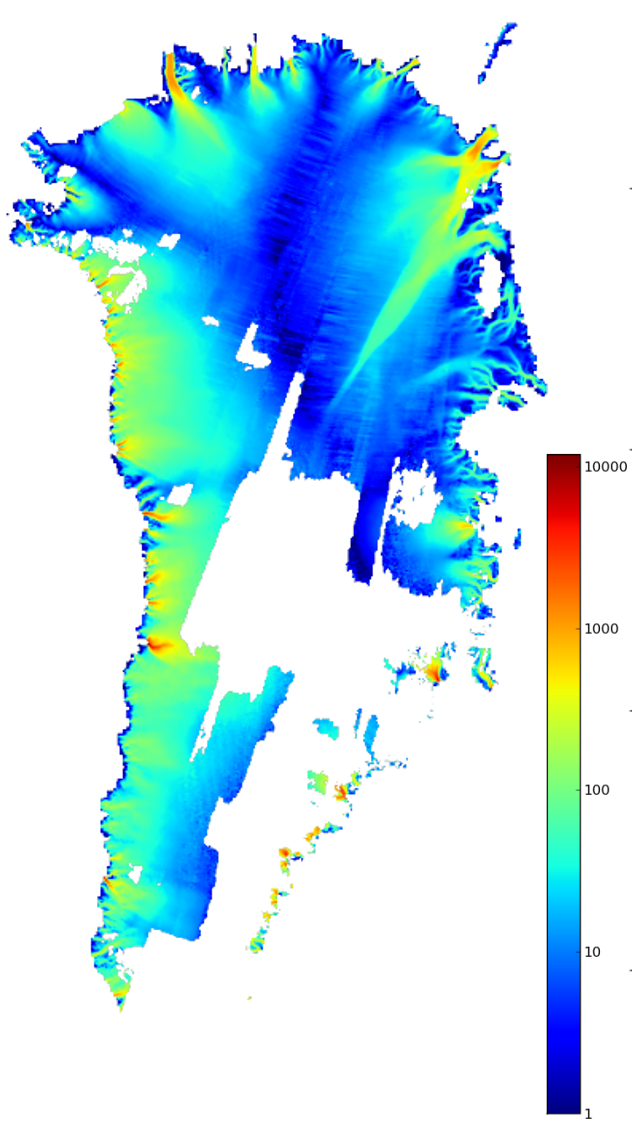
\includegraphics[height=0.85\textheight]{joughin}
\end{center}
\end{frame}


\begin{frame}
  \frametitle{Extra: Control run results 4: what happened at 20 model years?}

\begin{itemize}
\item previous results were at 100 model years; here is an example at 20 model years
\end{itemize}

\begin{center}
control run at 100 a \hfill control run at 20 a
\end{center}

\begin{columns}
\begin{column}{0.5\textwidth}
\scriptsize
\begin{center}
  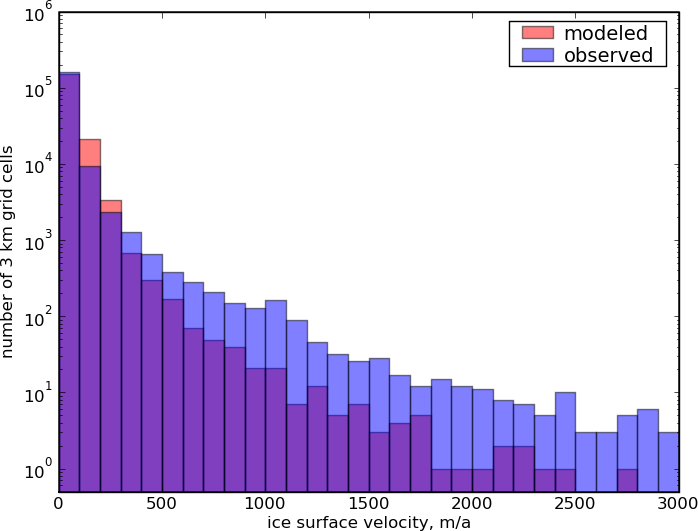
\includegraphics[width=0.9\textwidth]{g3km_3_25_98_hist}
\end{center}
\end{column}
\begin{column}{0.5\textwidth}
\begin{center}
  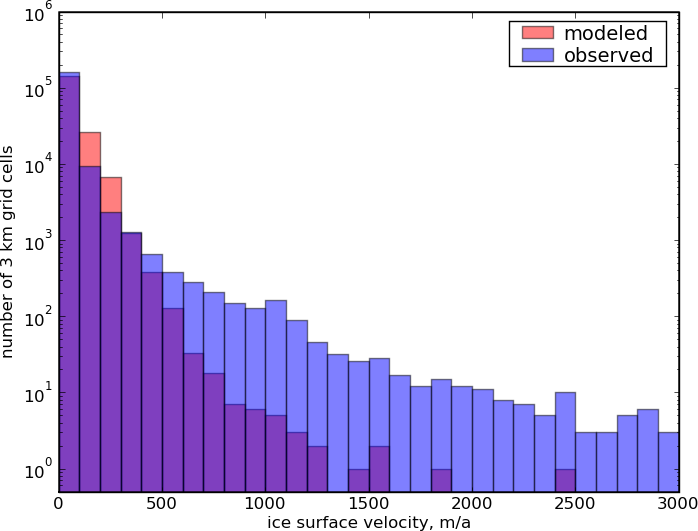
\includegraphics[width=0.9\textwidth]{g3km_3_25_98_early_hist}
\end{center}
\end{column}
\end{columns}
\end{frame}

\begin{frame}
  \frametitle{Extra: Geothermal high at source of NE Greenland}

\begin{itemize}\small
\item following Fahnestock et al (2001), try a 970 mW m-2 ``hot spot''
\end{itemize}
\vspace{-0.1in}

\begin{center}
control \hfill hotspot \hfill observed
\end{center}
\vspace{-0.15in}

\begin{columns}
\begin{column}{0.33\textwidth}
\begin{center}
  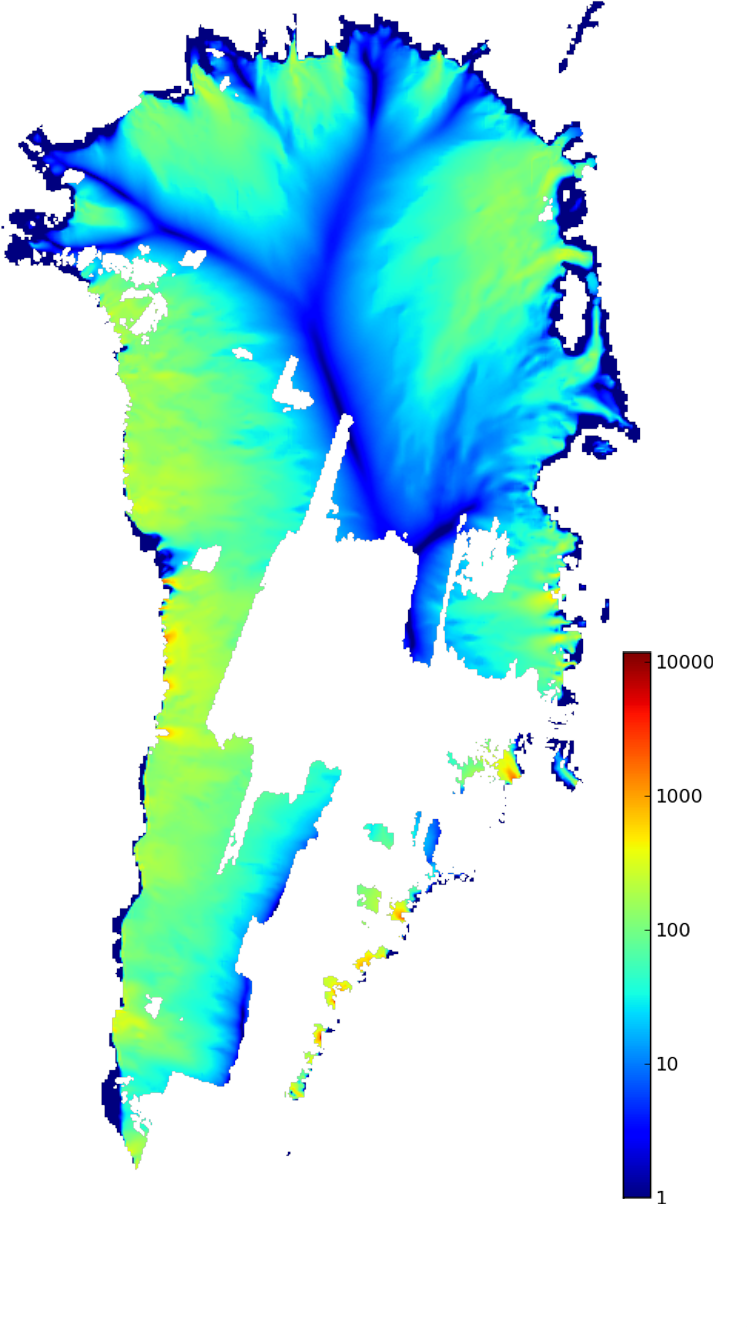
\includegraphics[width=0.75\textwidth]{g3km_3_25_98}
\end{center}
\end{column}
\begin{column}{0.33\textwidth}
\begin{center}
  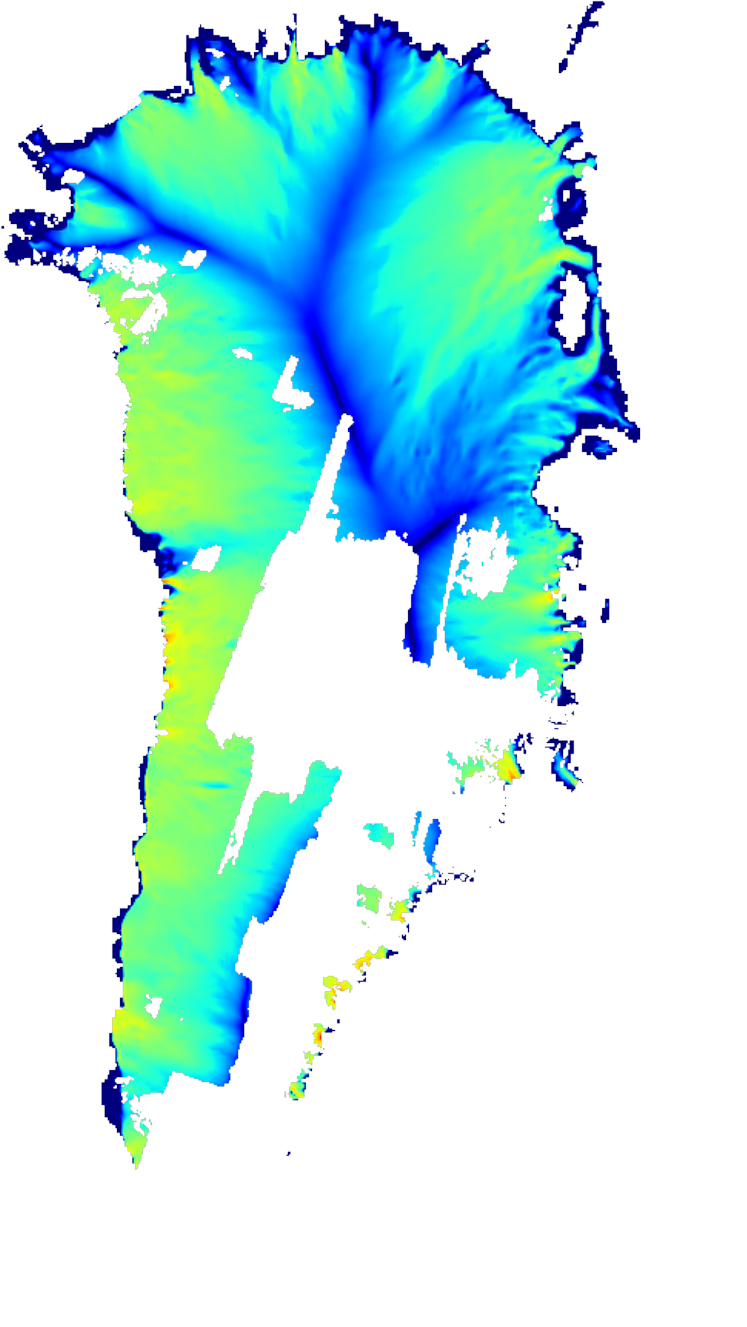
\includegraphics[width=0.75\textwidth]{g3km_3_25_98_hotspot}
\end{center}
\end{column}
\begin{column}{0.33\textwidth}
\begin{center}
  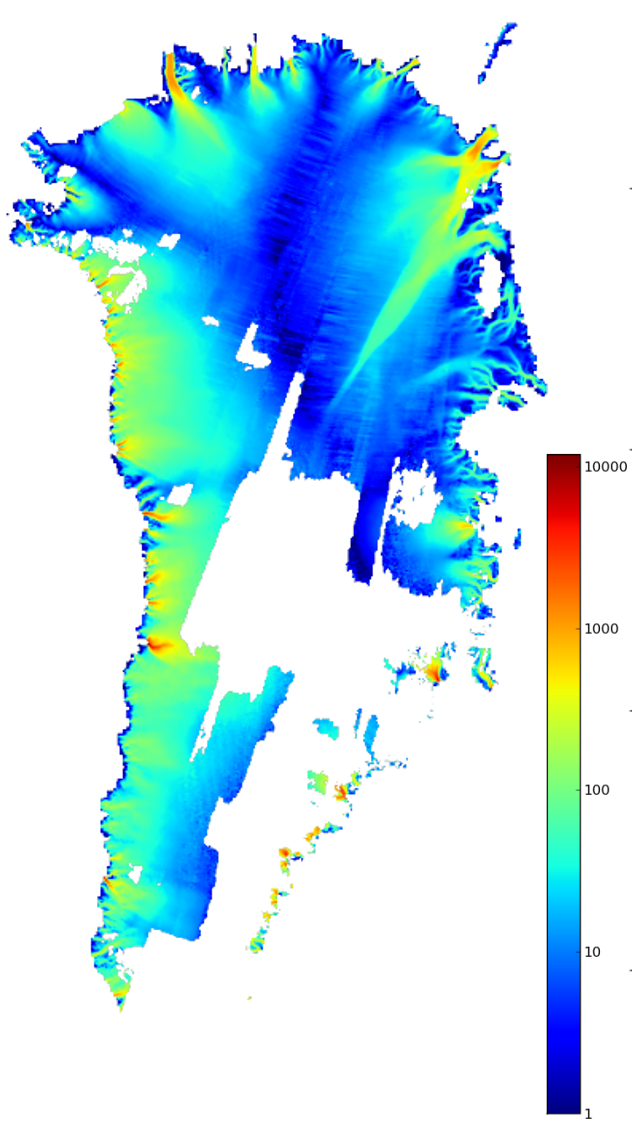
\includegraphics[width=0.75\textwidth]{joughin}
\end{center}
\end{column}
\end{columns}
\end{frame}


\begin{frame}
  \frametitle{PISM, cont.}

\begin{itemize}
\item verifiability
  \begin{itemize}
  \item construction of verification tests main focus during development (Bueler et al.~2005,2007)
  \item tests for SIA, SSA, and thermo- components
  \item can be checked at any time
  \end{itemize} 

\item derivability
  \begin{itemize}
  \item its a big C++ program
  \item Potsdam group (Levermann et al.) has PISM-PIK Antarctic model with improved ice shelf dynamics and fracture-based calving
  \end{itemize} 
\end{itemize} 
\end{frame}


\begin{frame}
  \frametitle{PISM: polythermal by enthalpy method 2}

\small
\begin{itemize}
\item conductivity of polythermal ice:
	$$k = \begin{cases}
	k_{\text{ice}}, & T(E,p) < T_{\text{pmp}}\\
	0, & T(E,p) = T_{\text{pmp}}
	\end{cases}$$
\item flow law is Paterson \& Budd (1982) with Lliboutry \& Duval (1985) dependence on $\omega$
\item cold-temperate transition surface (CTS) is boundary of $\omega > 0$ region
\item \dots so we have no explicit representation of CTS as a surface
\item \dots and no restriction on evolving CTS shape
\end{itemize}
\vspace{0.2in}

\begin{center}
  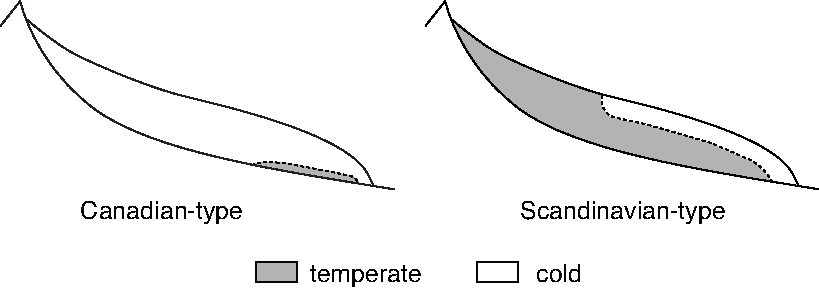
\includegraphics[width=0.6\textwidth]{polythermal_types}
\end{center}
\end{frame}



\end{document}

